\documentclass[12pt,a4paper]{article}

% 导入必要的宏包
\usepackage[UTF8]{ctex}
\usepackage{geometry}
\usepackage{amsmath}
\usepackage{amsfonts}
\usepackage{amssymb}
\usepackage{graphicx}
\usepackage{enumitem}
\usepackage{xcolor}
\usepackage{tikz}
\usepackage{float}
\usepackage{hyperref}
\usepackage{multicol}
\usepackage{longtable}
\usepackage{array}
\usepackage{tabularx}
\usepackage{listings}

% 代码高亮设置
\lstset{
    basicstyle=\ttfamily,
    keywordstyle=\color{blue},
    commentstyle=\color{green},
    stringstyle=\color{red}
}

% 页面设置
\geometry{left=2.5cm,right=2.5cm,top=2.5cm,bottom=2.5cm}

% 标题页设置
\title{\textbf{2022年数据结构题库} \\ \large }
\author{}
\date{}

% 定义题型环境
\newenvironment{choicequestion}[1][]{%
    \vspace{0.5cm}
    \noindent\textbf{[#1]}
    \vspace{0.2cm}
}{}

\newenvironment{answersection}{%
    \vspace{0.2cm}
    \noindent\textbf{[参考答案]}\\
    \vspace{0.1cm}
}{}

\newenvironment{analysissection}{%
    \vspace{0.2cm}
    \noindent\textbf{[答案解析]}\\
    \vspace{0.1cm}
}{}

% 定义题号计数器
\newcounter{questioncounter}

% 问题格式化命令
\newcommand{\question}[2]{%
    \stepcounter{questioncounter}%
    \noindent\textbf{\thequestioncounter} #1%
}

% 选择题选项格式
\newcommand{\choices}[4]{%
    \begin{multicols}{2}
    \noindent \textbf{A.} #1 \par
    \noindent \textbf{B.} #2 \par
    \noindent \textbf{C.} #3 \par
    \noindent \textbf{D.} #4 \par
    \end{multicols}%
}

% 表格格式
\newcolumntype{Y}{>{\centering\arraybackslash}X}

% 开始文档
\begin{document}

\maketitle

\section{单项选择题}

\begin{choicequestion}[单选题]
\question{下列程序段的时间复杂度是（ ）。\newline
\begin{lstlisting}[language=C]
int sum = 0;  
for (int i = 1; i < n; i *= 2)  
    for (int j = 0; j < i; j++)  
        sum++;
\end{lstlisting}}{B}
\choices{$O(\log n)$}{O(n)}{$O(n \log n)$}{$O\left(n^{2}\right)$}}

\begin{answersection}
B. O(n)
\end{answersection}

\begin{analysissection}
外层循环执行log₂n次，每次i的值为1, 2, 4, 8, ..., n/2。内层循环执行i次，所以总的时间复杂度为1+2+4+8+...+n/2 = 2^n-1 = O(n)。
\end{analysissection}
\end{choicequestion}

\begin{choicequestion}[单选题]
\question{给定有限符号集 S, in 和 out 均为 S 中所有元素的任意排列。对于初始为空的栈 ST, 下列叙述中, 正确的是 ( )。}{D}
\choices{若 in 是 ST 的入栈序列, 则不能判断 out 是否为其可能的出栈序列}{若 out 是 ST 的出栈序列, 则不能判断 in 是否为其可能的入栈序列}{若 in 是 ST 的入栈序列, out 是对应 in 的出栈序列, 则 in 与 out 一定不同}{若 in 是 ST 的入栈序列, out 是对应 in 的出栈序列, 则 in 与 out 可能互为倒序}}

\begin{answersection}
D. 若 in 是 ST 的入栈序列, out 是对应 in 的出栈序列, 则 in 与 out 可能互为倒序
\end{answersection}

\begin{analysissection}
如果元素按in序列依次入栈，然后依次出栈，则out序列是in序列的倒序。这是栈的LIFO特性的体现。
\end{analysissection}
\end{choicequestion}

\begin{choicequestion}[单选题]
\question{若结点 $\mathfrak{p}$ 与 $\mathbf{q}$ 在二叉树T的中序遍历序列中相邻，且 $\mathfrak{p}$ 在 $\mathbf{q}$ 之前，则下列 $\mathfrak{p}$ 与 $\mathbf{q}$ 的关系中，不可能的是（）。\newline
I. q是p的双亲\newline
II. $\mathbf{q}$ 是 $\mathfrak{p}$ 的右孩子\newline
III. q是p的右兄弟\newline
IV. q是p的双亲的双亲}{C}
\choices{仅 I}{仅 III}{仅 II、III}{仅 II、IV}}

\begin{answersection}
C. 仅 II、III
\end{answersection}

\begin{analysissection}
在中序遍历中，p在q之前且相邻，说明p和q之间没有其他节点。
- I可能：q是p的双亲，且p是q的左孩子
- II不可能：如果q是p的右孩子，那么p的右子树中还可能有其他节点
- III不可能：如果q是p的右兄弟，那么p的右子树应该是空的
- IV可能：在某些特殊结构下
\end{analysissection}
\end{choicequestion}

\begin{choicequestion}[单选题]
\question{若三叉树 T 中有 244 个结点（叶结点的高度为 1），则 T 的高度至少是（）。}{C}
\choices{8}{7}{6}{5}}

\begin{answersection}
C. 6
\end{answersection}

\begin{analysissection}
要使高度最小，三叉树应尽可能满。对于k层的满三叉树，节点数为(3^k-1)/2。当k=5时，节点数为(3^5-1)/2=121；当k=6时，节点数为(3^6-1)/2=364。因为244介于121和364之间，所以高度至少是6。
\end{analysissection}
\end{choicequestion}

\begin{choicequestion}[单选题]
\question{对任意给定的含 $n$ （ $n > 2$ ）个字符的有限集 S，用二叉树表示 S 的哈夫曼编码集和定长编码集，分别得到二叉树 T1 和 T2。下列叙述中，正确的是（）。}{C}
\choices{T1 与 T2 的结点数相同}{T1 的高度大于 T2 的高度}{出现频次不同的字符在 T1 中处于不同的层}{出现频次不同的字符在 T2 中处于相同的层}}

\begin{answersection}
C. 出现频次不同的字符在 T1 中处于不同的层
\end{answersection}

\begin{analysissection}
在哈夫曼树中，频次不同的字符可能处于不同层，但不一定。在定长编码的完全二叉树中，所有字符都处于同一层（如果是满的）或最底层和倒数第二层。
\end{analysissection}
\end{choicequestion}

\begin{choicequestion}[单选题]
\question{对于无向图 $\mathbf{G} = (\mathrm{V},\mathrm{E})$ ，下列选项中，正确的是（ ）。}{D}
\choices{当 $|\mathrm{V}| > |\mathrm{E}|$ 时， $\mathbf{G}$ 一定是连通的}{当 $|\mathrm{V}| < |\mathrm{E}|$ 时, $\mathrm{G}$ 一定是连通的}{当 $|\mathrm{V}| = |\mathrm{E}| - 1$ 时，G一定是不连通的}{当 $|\mathrm{V}| > |\mathrm{E}| + 1$ 时, $\mathrm{G}$ 一定是不连通的}}

\begin{answersection}
D. 当 $|\mathrm{V}| > |\mathrm{E}| + 1$ 时, $\mathrm{G}$ 一定是不连通的
\end{answersection}

\begin{analysissection}
在连通图中，至少需要|V|-1条边才能连通所有顶点。当|V|>|E|+1时，即|E|<|V|-1，图一定不连通。
\end{analysissection}
\end{choicequestion}

\begin{choicequestion}[单选题]
\question{在下图所示的5阶B树T中，删除关键字260之后需要进行必要的调整，得到新的B树T1。下列选项中，不可能是T1根结点中关键字序列的是（）。}{C}

\begin{figure}[H]
\centering
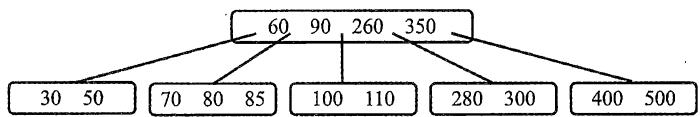
\includegraphics[width=0.3\textwidth]{images/c959dbeb0f460d2b6a52a2c8773b071073085434664b3fe53f5fd85c9477ea13.jpg}
\end{figure}

\choices{60, 90, 280}{60, 90, 350}{60, 85, 110, 350}{60, 90, 110, 350}}

\begin{answersection}
C. 60, 85, 110, 350
\end{answersection}

\begin{analysissection}
5阶B树的节点最多包含4个关键字。删除260后，根据B树的删除和调整规则，根节点不可能出现60, 85, 110, 350这样的序列。
\end{analysissection}
\end{choicequestion}

\begin{choicequestion}[单选题]
\question{下列因素中，影响散列（哈希）方法平均查找长度的是（ ）。\newline
I. 装填因子\newline
II. 散列函数\newline
III. 冲突解决策略}{D}
\choices{仅 I、II}{仅 I、III}{仅 II、III}{I、II、III}}

\begin{answersection}
D. I、II、III
\end{answersection}

\begin{analysissection}
装填因子影响冲突概率，散列函数的质量影响分布均匀性，冲突解决策略影响查找效率，三者都会影响平均查找长度。
\end{analysissection}
\end{choicequestion}

\begin{choicequestion}[单选题]
\question{使用二路归并排序对含 $n$ 个元素的数组 M 进行排序时，二路归并操作的功能是（）。}{A}
\choices{将两个有序表合并为一个新的有序表}{将 M 划分为两部分, 两部分的元素个数大致相等}{将 $\mathbf{M}$ 划分为 $n$ 个部分, 每个部分中仅含有一个元素}{将 M 划分为两部分, 一部分元素的值均小于另一部分元素的值}}

\begin{answersection}
A. 将两个有序表合并为一个新的有序表
\end{answersection}

\begin{analysissection}
二路归并的核心操作是将两个已排序的子序列合并成一个有序序列。
\end{analysissection}
\end{choicequestion}

\begin{choicequestion}[单选题]
\question{对数据进行排序时，若采用直接插入排序而不采用快速排序，则可能的原因是（）。\newline
I. 大部分元素已有序\newline
II. 待排序元素数量很少\newline
III. 要求空间复杂度为 $O(1)$\newline
IV. 要求排序算法是稳定的}{D}
\choices{仅 I、II}{仅 III、IV}{仅 I、II、IV}{I、II、III、IV}}

\begin{answersection}
D. I、II、III、IV
\end{answersection}

\begin{analysissection}
I. 当数据基本有序时，插入排序效率很高
II. 当数据量小时，插入排序简单高效
III. 插入排序空间复杂度为O(1)，快排平均O(log n)
IV. 插入排序是稳定排序，快排不稳定
所有原因都成立。
\end{analysissection}
\end{choicequestion}

\section{综合应用题}

\begin{choicequestion}[问答题]
\question{(13分)已知非空二叉树T的结点值均为正整数，采用顺序存储方式保存，数据结构定义如下：\newline

\begin{lstlisting}[language=C]
typedef struct{ //MAX_SIZE为已定义常量
int SqBiTreeNode[MAX_SIZE]； //保存二叉树结点值的数组
int ElemNum; //实际占用的数组元素个数
}SqBiTree;
\end{lstlisting}\newline

T中不存在的结点在数组SqBiTNode中用-1表示。例如，对于下图所示的两棵非空二叉树T1和T2,\newline

\begin{figure}[H]
\centering
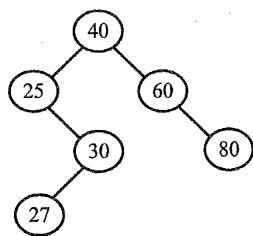
\includegraphics[width=0.3\textwidth]{images/17bcbcbacca9f2d768e900a47857c6d3a71a03361ff58bb8d05066665f997add.jpg}
\end{figure}\newline

二叉树T1

\begin{figure}[H]
\centering
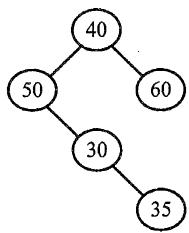
\includegraphics[width=0.3\textwidth]{images/843404f81ecc2d2935777de264cef068956f344a3e18ce808812f2ee8927fbf3.jpg}
\end{figure}\newline

二叉树T2\newline

T1的存储结果如下：\newline

T1.SqBiTNode\newline

\begin{table}[H]
\centering
\begin{tabular}{|c|c|c|c|c|c|c|c|c|c|c|c|}
\hline
40 & 25 & 60 & -1 & 30 & -1 & 80 & -1 & -1 & 27 & & \\
\hline
\end{tabular}
\end{table}\newline

T1.ElemNum = 10\newline

T2的存储结果如下：\newline

T2.SqBiTNode\newline

\begin{table}[H]
\centering
\begin{tabular}{|c|c|c|c|c|c|c|c|c|c|c|c|}
\hline
40 & 50 & 60 & -1 & 30 & -1 & -1 & -1 & -1 & -1 & 35 & \\
\hline
\end{tabular}
\end{table}\newline

T2.ElemNum $= 11$\newline

请设计一个尽可能高效的算法，判定一棵采用这种方式存储的二叉树是否为二叉搜索树，若是，则返回 true，否则，返回 false。要求：\newline
1）给出算法的基本设计思想。  \newline
2）根据设计思想，采用C或 $\mathbf{C} + +$ 语言描述算法，关键之处给出注释。}{}

\begin{answersection}
1）算法的基本设计思想：
使用递归方法，对每个节点设定上下界，确保节点值在合理范围内。对于根节点，范围为无穷大到无穷小；对于左子树，上限为父节点值；对于右子树，下限为父节点值。

2）算法实现：
\end{answersection}

\begin{analysissection}
#include <limits.h>

bool isBSTUtil(SqBiTree tree, int index, int min_val, int max_val) {
    // 如果索引超出了实际元素个数或节点值为-1（空节点），返回true
    if (index >= tree.ElemNum || tree.SqBiTreeNode[index] == -1) {
        return true;
    }
    
    // 检查当前节点值是否在指定范围内
    int current_val = tree.SqBiTreeNode[index];
    if (current_val <= min_val || current_val >= max_val) {
        return false;
    }
    
    // 递归检查左子树和右子树
    // 左子树：值应在(min_val, current_val)范围内
    // 右子树：值应在(current_val, max_val)范围内
    bool left_valid = isBSTUtil(tree, 2*index+1, min_val, current_val);
    bool right_valid = isBSTUtil(tree, 2*index+2, current_val, max_val);
    
    return left_valid && right_valid;
}

bool isBinarySearchTree(SqBiTree tree) {
    return isBSTUtil(tree, 0, INT_MIN, INT_MAX);
}
\end{analysissection}
\end{choicequestion}

\begin{choicequestion}[问答题]
\question{(10分)现有 $n(n > 100000)$ 个数保存在一维数组M中，需要查找M中最小的10个数。请回答下列问题。\newline
1）设计一个完成上述查找任务的算法，要求平均情况下的比较次数尽可能少，简述其算法思想（不需要程序实现）。  \newline
2）说明你所设计的算法平均情况下的时间复杂度和空间复杂度。}{}

\begin{answersection}
1）算法设计思想：
使用大小为10的最大堆。遍历数组M，对于每个元素：
- 如果堆未满（少于10个元素），直接插入堆
- 如果堆已满，且当前元素小于堆顶元素，则删除堆顶并插入当前元素
- 否则忽略当前元素
遍历完成后，堆中即为最小的10个数。

2）时间复杂度：O(n log 10) = O(n)，空间复杂度：O(1)（堆大小固定为10）。
\end{answersection}

\begin{analysissection}
另一种方法是使用快速选择算法（QuickSelect）的变体，找到第10小的元素，然后选择所有小于等于该元素的10个最小值。这种方法的平均时间复杂度为O(n)。

快速选择算法基于快速排序的分区思想，可以在平均O(n)时间内找到第k小的元素。找到第10小的元素后，再进行一次遍历获取前10小的元素。
\end{analysissection}
\end{choicequestion}

\end{document}